\documentclass[aspectratio=169]{beamer}
\mode<presentation>{
    \usetheme{Frankfurt}
    \usecolortheme{rose}}
%%%%%%%%%%%%%%%%%%%%%%%%%%%%%%%%%%%%%%%%%%%%%%%%%%
\usepackage[utf8]{inputenc}
\usepackage[brazil]{babel}
\usepackage{graphicx} 
\usepackage{booktabs}
\usepackage{subcaption}
\usepackage{multirow}
\usepackage{xcolor}
\usepackage{amsthm}
\usepackage{amssymb}
\usepackage{amsmath}    
\usepackage{listings}
\usepackage{longtable}
\usepackage{lscape}
\usepackage[T1]{fontenc}
\usepackage{txfonts}
\usepackage{ragged2e}
\usepackage{etoolbox}
\usepackage{hyperref}   
\usepackage{transparent}
\usepackage{epstopdf}
\usepackage{enumerate}
\usepackage{multicol}
\usepackage{ragged2e}
%%%%%%%%%%%%%%%%%%%%%%%%%%%%%%%%%%%%%%%%%%%%%%%%%%
\newcommand{\Vv}{\overline{v}}%Letra v de solução
\newcommand{\Ww}{\overline{w}}%Letra w de solução
\newcommand{\kk}{\kappa}%Letra kappa
\newcommand{\cc}{\lambda}%Letra lambda
\newcommand{\ct}{\widetilde{C}}%Letra c com tiu
\newcommand{\zz}{{\mathbf{z}}}%Letra z de campo vetorial
\newcommand{\vv}{\nu}%Letra nu
\newcommand{\pp}{\widetilde{p}}%Letra p com acento
\newcommand{\pc}{p^{*}}%Letra p conjugada
\newcommand{\dd}{{\hspace*{0.08cm}}{\mathrm{d}}}%Letra p conjugada
\newcommand{\MM}{{\mathcal{M}}}%Letra p conjugada
\newcommand{\IN}{{\scriptscriptstyle{N}}}%Letra p conjugada
% CONJUNTOS E ESPAÇOS
\newcommand{\DMIO}{{\mathcal{DM}}^\infty(\Omega)}
\newcommand{\BVo}{{BV}(\Omega)}%Espaço BV de Omega
\newcommand{\IBV}{_{\scriptscriptstyle{BV}}}%Indice BV
\newcommand{\BVloc}{{BV}_{loc}(\Omega)}%Espaço BV de Omega
\newcommand{\LpO}{{L}^p(\Omega)}%Espaço L p de Omega
\newcommand{\ILp}{_{\scriptscriptstyle{L}^p}}%Indice L p 
\newcommand{\Linfo}{\emph{L}^\infty(\Omega)}%L infinito de Omega
\newcommand{\Linforn}{{L}^\infty(\Omega,{\mathbb{R}}^N)}%L infitiro de Omega em Rn
\newcommand{\ILinf}{_{\scriptscriptstyle{{L}}^\infty}}%L infitiro de Omega em Rn
\newcommand{\LUmO}{{\emph{L}}^1(\Omega)}%Espaço L 1 de Omega
\newcommand{\ILUmO}{_{\scriptscriptstyle{\emph{L}}^1(\Omega)}}%Indice L 1 de Omega
\newcommand{\ILUm}{_{\scriptscriptstyle{L}^1}}%Indice L 1 de Omega
\newcommand{\Diso}{{\mathcal{D}}^\prime(\Omega)}%Espaço das distribuições em Omega 
\newcommand{\IDis}{_{\scriptscriptstyle{\mathcal{D}}^\prime}}%Espaço das distribuições em Omega
\newcommand{\WumpzO}{{W}^{1,p}_0(\Omega)}%Espaço das W 1 p 0 de Omega
\newcommand{\IWumpz}{_{\scriptscriptstyle{W}^{1,p}_0} }%Indice do espaço das W 1 p 0
\newcommand{\WumpO}{{W}^{1,p}(\Omega)}%Espaço das W 1 p de Omega
\newcommand{\CUmCO}{{\mathcal{C}}^{1}_0(\Omega)}%Espaço C Um com suporte Compacto em Omega
\newcommand{\ICUmC}{_{\scriptscriptstyle{\mathcal{C}}^{1}_0}}%Espaço C Um com suporte Compacto em Omega
\newcommand{\CInfZO}{{\mathcal{C}}^{\infty}_0(\Omega)}% EspaçoC infinito de 0 em Omega
\newcommand{\CInfCO}{{\mathcal{C}}^{\infty}_0(\Omega)}% EspaçoC infinito de 0 em Omega
\newcommand{\CInfO}{{\mathcal{C}}^{\infty}(\Omega)}% EspaçoC infinito em Omega
\newcommand{\CO}{{\mathcal{C}}(\Omega)}
\newcommand{\ICInfZ}{_{\scriptscriptstyle{\mathcal{C}}^{\infty}_0}}% Indice C infinito de 0
\newcommand{\Cc}{{\mathbb{C}}}%Conjunto dos complexos
\newcommand{\Rr}{{\mathbb{R}}}%Conjunto dos Reais
\newcommand{\Nn}{{\mathbb{N}}}%Conjunto dos naturais
\newcommand{\DDo}{{\mathcal{D}}(\Omega)}%Espaço das funções testes
% OPERADORES
\newcommand{\sign}{{\text{sign}}}%Operador sign   
\newcommand{\dive}{{\text{div}}}%Operador divergente
\newcommand{\umlapla}{\text{div}\left(\dfrac{Du}{\left|Du\right| } \right)}%aOperador 1-laplaciano
\newcommand{\IntO}{\displaystyle\int_\Omega}%Integral sobre omega
\newcommand{\IntFO}{\displaystyle\int_{\partial\Omega}}%Integral sobre a fronteira de omega
\newcommand{\IntZS}{\displaystyle\int_{0}^s}%Integral de 0 a s
\newcommand{\IntSzS}{\displaystyle\int_{s_0}^s}%Integral de s_0 a s
\newcommand{\IntZSz}{\displaystyle\int_{0}^{s_0}}%Integral de 0 a s_0
\newcommand{\MedH}{{\mathcal{H}}^{N-1}}%Medida de Hausdorf de N-1
\newcommand{\Deln}{\Delta}
\newcommand{\Deli}{\nabla}
\newcommand{\ComO}{\left|\Omega\right| }
\newcommand{\supp}{{\text{supp}}}%Operador suporte

\newcommand{\liminfpum}{{\liminf\limits_{p\to 1^+}}}
\newcommand{\limsuppum}{{\limsup\limits_{p\to 1^+}}}
\newcommand{\limsups}{{\limsup\limits_{s\to 0}}}
\newcommand{\Impli}{\Rightarrow}
\newcommand{\Vai}{\longrightarrow}
\newcommand{\Chega}{\longmapsto}
\newcommand{\ToFr}{\rightharpoonup}

\newcommand{\Moe}{\left|}
\newcommand{\Mod}{\right|}
\newcommand{\Noe}{\left\|}
\newcommand{\Nod}{\right\|}
\newcommand{\NBVe}{\left|\hspace*{-0.05cm}\left|\hspace*{-0.05cm}\left|}
\newcommand{\NBVd}{\right|\hspace*{-0.05cm}\right|\hspace*{-0.05cm}\right|\IBV}
\newcommand{\Pae}{\left( }
\newcommand{\Pad}{\right) }
\newcommand{\Poe}{\left\langle}
\newcommand{\Pod}{\right\rangle}
\newcommand{\Que}{\left[}
\newcommand{\Qud}{\right] }

\setbeamertemplate{theorems}[ams style]
\newtheorem{ter}{Teorema}
\newtheorem{terr}{Teorema}
\newtheorem{defin}{Definição}
\newtheorem{lema}{Lema}
\newtheorem{obs}{Observação}
\newtheorem{prop}{Proposição}
\newtheorem{exem}{Exemplo}

%%%%%%%%%%%%%%%%%%%%%%%%%%%%%%%%%%%%%%%%%%%%%%%%%%
% Logo: O comando original procurava um arquivo "Logo.png" e causava erro se não existisse.
% Foi substituído por uma caixa de espaço como solicitado. Quando tiver o arquivo, use o comando abaixo:
% \titlegraphic{\hfill
\includegraphics[height=1.5cm]{Logo.png}}
\titlegraphic{
    \begin{center}
        
\includegraphics[width=3.5cm]{pic/AVVR03.eps}
    \end{center}
}
\title{Grandes Modelos de Linguagem}
\author[Exame de Qualificação]{\textbf{Alunos:} João Gabriel de Morais Bezerra e Daniel Henrique Peres Servejeira}%\\ \textbf{Orientador:} Prof. Dr. Cássio Machiaveli Oishi} 
\institute{Laboratório de Simulações Numéricas e Inteligência Artificial}
\date{\today}
%%%%%%%%%%%%%%%%%%%%%%%%%%%%%%%%%%%%%%%%%%%%%%%%%%
\begin{document}
%%%%%%%%%%%%%%%%%%%%%%%%%%%%%%%%%%%%%%%%%%%%%%%%%%
\begin{frame}
    \titlepage{}
\end{frame}
%%%%%%%%%%%%%%%%%%%%%%%%%%%%%%%%%%%%%%%%%%%%%%%%%%
\section{Introdução}

\begin{frame}{Modelos de linguagem}\justifying
    \textbf{Lembre-se do modelo de linguagem simples n-grama:}
    \begin{itemize}
        \item Atribui probabilidades a sequências de palavras;
        \item Gera texto amostrando possíveis próximas palavras;
        \item É treinado em contagens de frequência computadas a partir de corpora textuais massivos.
    \end{itemize}
    \vspace{0.5cm}
    \textbf{Grandes modelos de linguagem compartilham semelhanças, mas diferem fundamentalmente:}
    \begin{itemize}
        \item Atribuem probabilidades a sequências de palavras;
        \item Geram texto amostrando possíveis próximas palavras;
        \item São treinados utilizando redes neurais profundas para aprender a adivinhar a próxima palavra.
    \end{itemize}
\end{frame}

\begin{frame}{Grandes modelos de linguagem}\justifying
    Mesmo que esses modelos complexos sejam pré-treinados exclusivamente com o objetivo simples de prever a próxima palavra sequencial, eles implicitamente aprendem uma quantidade massiva de estrutura linguística útil, conhecimento factual e capacidades de raciocínio devido à escala astronômica dos textos que processam durante o treinamento.
\end{frame}

\begin{frame}{Três arquiteturas para grandes modelos de linguagem}\justifying
    \begin{columns}[t]
        \begin{column}{0.33\textwidth}
            \textbf{Decodificadores}
            \begin{itemize}
                \item GPT Series
                \item Claude
                \item Llama
                \item Mixtral
            \end{itemize}
        \end{column}

        \begin{column}{0.33\textwidth}
            \textbf{Codificadores}
            \begin{itemize}
                \item BERT family
                \item HUBERT
            \end{itemize}
        \end{column}

        \begin{column}{0.33\textwidth}
            \textbf{Codificadores-Decodificadores}
            \begin{itemize}
                \item Flan-T5
                \item Whisper
            \end{itemize}
        \end{column}
    \end{columns}

    \vspace{0.5cm}

    \begin{columns}[c]
        \begin{column}{0.33\textwidth}
            \centering
            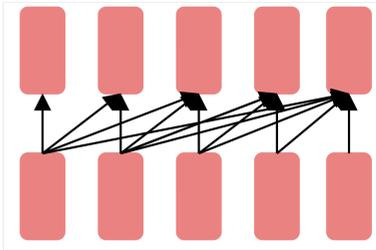
\includegraphics[width=0.5\linewidth]{pic/decoders.jpeg}
        \end{column}

        \begin{column}{0.33\textwidth}
            \centering
            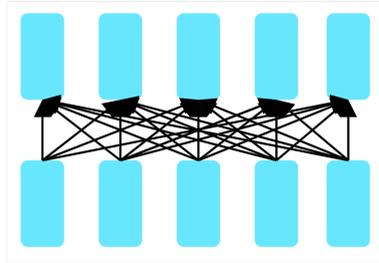
\includegraphics[width=0.5\linewidth]{pic/encoders.jpeg}
        \end{column}

        \begin{column}{0.33\textwidth}
            \centering
            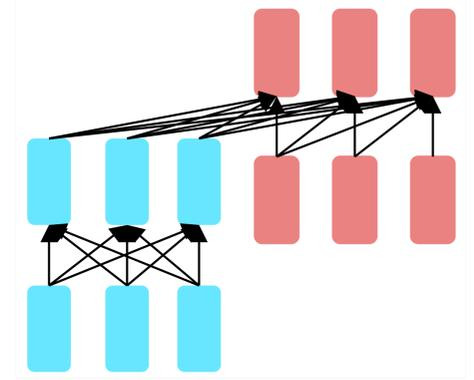
\includegraphics[width=0.7\linewidth]{pic/encoders-decoders.jpeg}
        \end{column}
    \end{columns}
\end{frame}

\begin{frame}{Codificadores}\justifying
    \textbf{Muitas variedades existem no ecossistema:}
    \begin{itemize}
        \item Variante mais popular: Modelos de Linguagem Mascarada (MLMs), como a família BERT.
        \item Treinados prevendo palavras que foram artificialmente mascaradas do contexto ao redor em ambos os lados, esquerdo e direito.
        \item Por serem bidirecionais, eles geralmente passam por um ajuste fino (treinados em dados supervisionados) exclusivamente para tarefas de classificação e extração em vez de geração.
    \end{itemize}
    \vspace{0.2cm}
    \begin{figure}
        \centering
        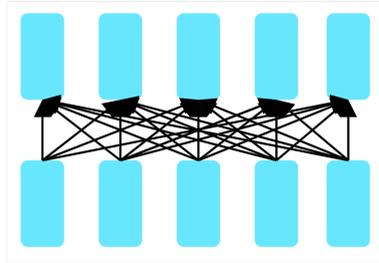
\includegraphics[width=0.3\linewidth]{pic/encoders.jpeg}
        \label{fig:encoders}
    \end{figure}
\end{frame}

\begin{frame}{Codificadores-Decodificadores}\justifying
    \textbf{Treinados fundamentalmente para mapear de uma sequência completa para outra.} \\
    \vspace{0.2cm}
    \textbf{Muito populares para tarefas que requerem compreensão total do contexto:}
    \begin{itemize}
        \item Tradução automática (mapear uma frase inteiramente de um idioma para outro)
        \item Reconhecimento de fala (mapear acústica de áudio bruto em palavras escritas)
    \end{itemize}
    \vspace{0.3cm}
    \begin{figure}
        \centering
        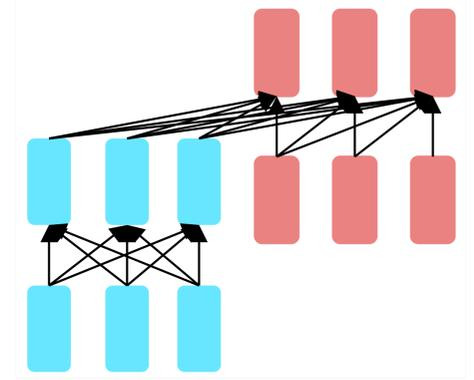
\includegraphics[width=0.3\linewidth]{pic/encoders-decoders.jpeg}
        \label{fig:encoders-decoders}
    \end{figure}
\end{frame}

%%%%%%%%%%%%%%%%%%%%%%%%%%%%%%%%%%%%%%%%%%%%%%%%%%
\section{Ger. Condicional}

\begin{frame}{Grandes Modelos de Linguagem}
    \begin{center}
        \huge \textbf{Grandes Modelos de Linguagem}\\
        \vspace{0.5cm}
        \Large Quais tarefas eles podem realizar?
    \end{center}
\end{frame}

\begin{frame}{A grande ideia}\justifying
    \Large
    Um avanço monumental no processamento de linguagem natural é a constatação de que muitas tarefas cognitivas complexas podem ser reformuladas matematicamente como tarefas simples de prever palavras!
\end{frame}

\begin{frame}{Nesta aula: modelos apenas decodificadores}\justifying
    \textbf{Modelos apenas decodificadores são comumente chamados de:}
    \begin{itemize}
        \item LLMs Causais
        \item LLMs Autorregressivos
        \item LLMs da Esquerda para a Direita
    \end{itemize}
    Esses modelos funcionam estritamente prevendo palavras sequencialmente da esquerda para a direita, sendo totalmente incapazes de analisar o contexto futuro.
\end{frame}

\begin{frame}{Geração Condicional}\justifying
    \textbf{Gerando texto logicamente condicionado ao texto anterior!}
    
    \vspace{0.5cm}
    \begin{figure}
        \centering
        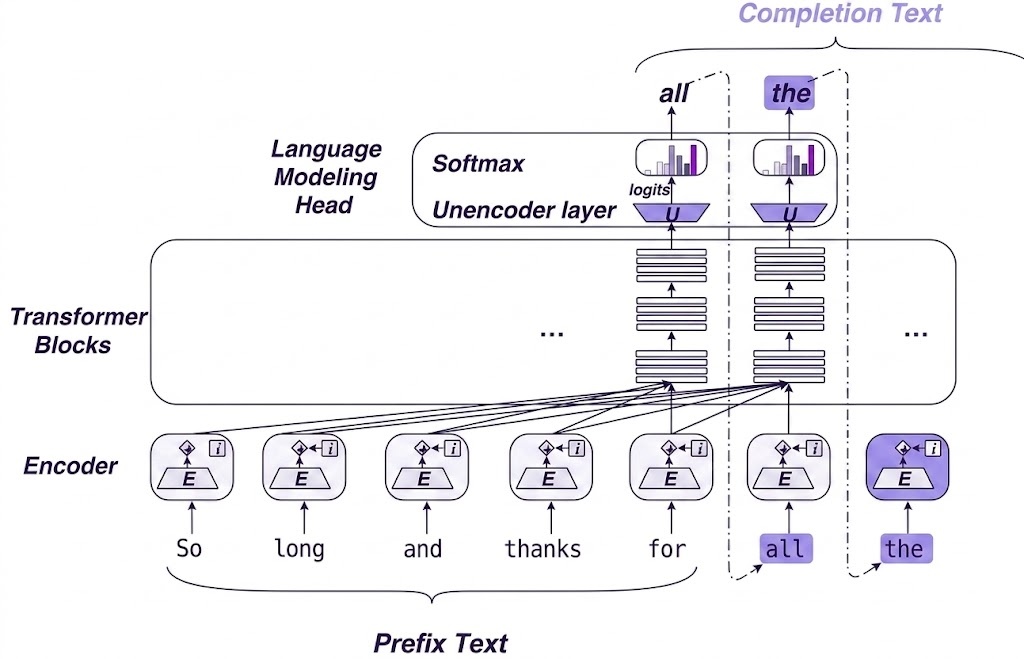
\includegraphics[width=0.6\linewidth]{pic/conditional-generation.png}
        \caption{Esquema de previsão de texto.}
        \label{fig:esquema_previsao_texto}
    \end{figure}
\end{frame}

\begin{frame}{Formulando muitas tarefas como previsão de palavras: Análise de Sentimentos}\justifying
    \textbf{Análise de sentimentos da frase: "Eu gosto do Jackie Chan"}
    
    \begin{enumerate}
        \item Nós fornecemos ao modelo de linguagem autorregressivo esta string de prefixo específica: \\
        \textit{O sentimento da frase "Eu gosto do Jackie Chan" é:}
        \item Em seguida, avaliamos a probabilidade matemática da palavra que ele acha que vem a seguir: \\
        \[ P(\text{positivo} \mid \text{prefixo}) \quad \text{versus} \quad P(\text{negativo} \mid \text{prefixo}) \]
    \end{enumerate}
    O modelo avalia as probabilidades de pares semânticos como gostar/odiar, amar/não gostar e adorar/detestar para executar a classificação.
\end{frame}

\begin{frame}{Formulando muitas tarefas como geração condicional: QA}\justifying
    \textbf{Perguntas e Respostas (QA): "Quem escreveu A Origem das Espécies"}
    
    \begin{enumerate}
        \item Damos ao modelo de linguagem esta string estrutural rigorosa: \\
        \texttt{P: Quem escreveu o livro "A Origem das Espécies"? R:}
        \item E avaliamos qual palavra a distribuição de probabilidade indica que virá a seguir.
        \item Anexamos o resultado e iteramos o processo: \\
        \texttt{P: Quem escreveu o livro "A Origem das Espécies"? R: Charles}
    \end{enumerate}
\end{frame}

\begin{frame}{Resumo via Geração Condicional}\justifying
    \textbf{Exemplo de Artigo Original:} \\
    A única coisa mais louca do que um cara na nevada Massachusetts empacotando aquela neve branquinha e oferecendo-a para venda online? As pessoas estão realmente comprando. Por US\$ 89, o auto-intitulado empreendedor Kyle Waring enviará cerca de 3 quilos de neve da área de Boston em uma caixa de isopor isolada - o suficiente para 10 a 15 bolas de neve, diz ele. Mas não se você mora na Nova Inglaterra ou nos estados vizinhos.
    
    \vspace{0.5cm}
    \textbf{Resumo Gerado (solicitado por "tl;dr"):} \\
    Kyle Waring enviará a você cerca de 3 quilos de neve da área de Boston em uma caixa isolada, o suficiente para 10 a 15 bolas de neve, diz ele. Mas não se você mora na Nova Inglaterra ou nos estados vizinhos. Ele brincou sobre enviar o material para amigos e familiares em estados mais quentes, e assim nasceu uma ideia.
\end{frame}

\begin{frame}{Sumarização de texto}\justifying
    \textbf{Executando compressão usando o delimitador "Too long; didn’t read".}
    \vspace{0.5cm}
    \begin{figure}
        \centering
        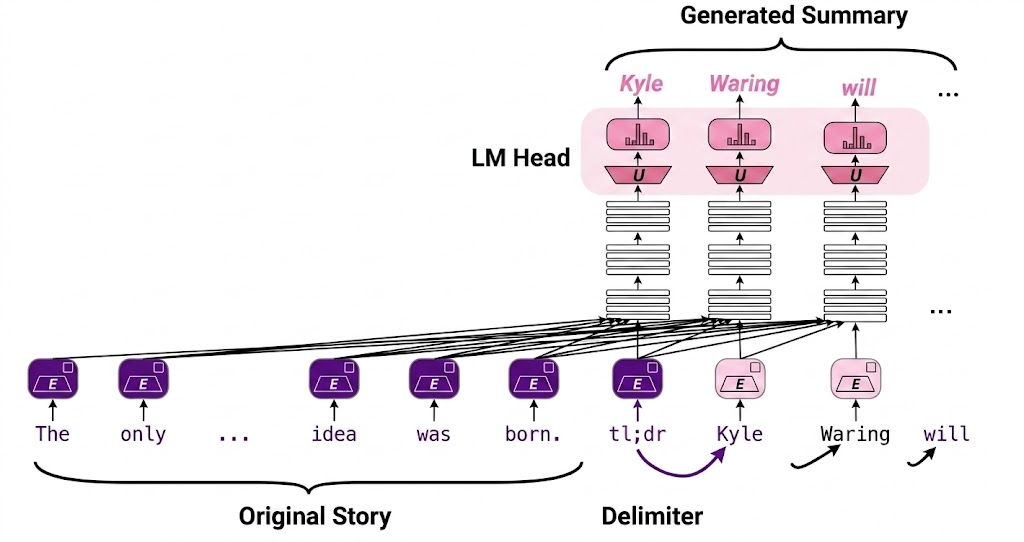
\includegraphics[width=0.7\linewidth]{pic/summarization.png}
        \caption{Esquema de resumo de texto.}
        \label{fig:esquema_resumo_texto}
    \end{figure}
    \vspace{2.5cm}
\end{frame}

%%%%%%%%%%%%%%%%%%%%%%%%%%%%%%%%%%%%%%%%%%%%%%%%%%
\section{Alg. de Dec. e Amostragem}

\begin{frame}{Amostragem para Geração de LLMs}
    \begin{center}
        \huge \textbf{Amostragem para Geração de LLMs}
    \end{center}
\end{frame}

\begin{frame}{Decodificação e Amostragem}\justifying
    \begin{itemize}
        \item A tarefa computacional de escolher uma palavra específica para gerar com base nas probabilidades de saída do modelo é chamada de \textbf{decodificação}.
        \item O método mais comum para decodificação em LLMs é a \textbf{amostragem}.
        \item Amostrar a partir da distribuição de palavras de um modelo envolve escolher palavras aleatórias de acordo com a probabilidade matemática precisa atribuída pela rede.
        \item Após cada token ser gerado, amostramos palavras subsequentes de acordo com sua probabilidade estritamente condicionada a todas as nossas escolhas anteriores.
        \item Um modelo de linguagem Transformer produzirá continuamente essa distribuição de probabilidade sobre o vocabulário.
    \end{itemize}
\end{frame}

\begin{frame}[fragile]{Amostragem aleatória}\justifying
    Intuição algorítmica para a amostragem aleatória pura:
    \vspace{0.5cm}
\begin{lstlisting}[language=Python, basicstyle=\ttfamily\small, backgroundcolor=\color{gray!10}, keywordstyle=\color{blue}]
i = 1
w_1 \leftarrow p(w)
while w_i!= EOS:
    i = i + 1
    w_i \leftarrow p(w | w_1,..., w_{i-1})
\end{lstlisting}
    \vspace{0.5cm}
    \begin{itemize}
        \item $i$ e $w_i$: Rastreiam o índice posicional e a palavra escolhida.
        \item $\leftarrow p$: Indica a extração probabilística da palavra a partir da distribuição.
        \item \textbf{EOS}: O sinal crítico de parada (Fim da Sequência).
        \item $P(w \mid \dots)$: A escolha da próxima palavra depende de todo o contexto histórico.
    \end{itemize}
\end{frame}

\begin{frame}{A amostragem aleatória não funciona muito bem...}\justifying
    \begin{itemize}
        \item Embora a amostragem aleatória pura geralmente gere palavras coerentes e de alta probabilidade, existem milhares de palavras estranhas e de baixa probabilidade residindo na cauda da distribuição.
        \item Cada uma dessas palavras individuais possui uma probabilidade mínima, mas quando somadas matematicamente, elas constituem uma parte grande e perigosa da massa de probabilidade total.
        \item Portanto, sob amostragem aleatória pura, elas são escolhidas com frequência suficiente para gerar frases completamente estranhas e sem sentido.
    \end{itemize}
\end{frame}

\begin{frame}{Fatores na amostragem de palavras: Qualidade vs. Diversidade}\justifying
    \textbf{Enfatizar palavras com probabilidade média introduz diversidade:}
    \begin{itemize}
        \item \textbf{Prós:} Resulta em saídas textuais muito mais criativas e diversas.
        \item \textbf{Contras:} Reduz drasticamente a qualidade, resultando em declarações menos factuais e altamente inconsistentes.
    \end{itemize}
    \vspace{0.5cm}
    \textbf{Enfatizar palavras exclusivamente com alta probabilidade prioriza a qualidade:}
    \begin{itemize}
        \item \textbf{Prós:} Garante que as saídas sejam altamente precisas, logicamente coerentes e factuais.
        \item \textbf{Contras:} Erradica a diversidade, produzindo textos entediantes, altamente repetitivos e robóticos.
    \end{itemize}
\end{frame}

\begin{frame}{Algoritmo de Amostragem Top-k}\justifying
    Para truncar a perigosa cauda de probabilidade, utilizamos o Top-k:
    \begin{enumerate}
        \item Escolha um valor inteiro estático "$k$" representando o número de palavras.
        \item Para cada palavra em todo o vocabulário $V$, use o modelo de linguagem para calcular a probabilidade dessa palavra dado o prefixo contextual $p(w_t \mid w_{<t})$.
        \item Ordene as palavras sequencialmente por probabilidade, mantendo apenas as "$k$" palavras mais prováveis e descartando o resto.
        \item Renormalize as pontuações das $k$ palavras restantes para que somem 1, criando uma distribuição de probabilidade válida.
        \item Selecione aleatoriamente uma palavra das $k$ palavras restantes, estritamente de acordo com sua probabilidade renormalizada.
    \end{enumerate}
\end{frame}

\begin{frame}{Amostragem Top-p (= amostragem de núcleo)}\justifying
    \textbf{Problema Fundamental com o top-k:} O parâmetro $k$ é fixo, o que significa que pode abranger quantidades muito diferentes da massa de probabilidade total em situações contextuais diferentes (por exemplo, distribuições planas vs. acentuadas). \\
    \vspace{0.3cm}
    \textbf{A Ideia do Núcleo:} Em vez de uma contagem fixa, mantenha os $p$ por cento superiores da massa de probabilidade. \\
    \vspace{0.3cm}
    Dada uma distribuição $P(w_t \mid w_{<t})$, o vocabulário top-p $V(p)$ é definido matematicamente como o menor conjunto de palavras tal que:
    \[ \sum_{w \in V(p)} P(w \mid w_{<t}) \ge p \]
    \vspace{0.3cm}
    \raggedleft \textit{(Holtzman et al., 2020)}
\end{frame}

\begin{frame}{Amostragem por temperatura (1/4)}\justifying
    Em vez de truncar o vocabulário, podemos remodelar matematicamente toda a distribuição. Esse conceito extrai intuição da termodinâmica:
    \begin{itemize}
        \item Um sistema físico existente a uma temperatura alta é altamente flexível, energético e pode explorar muitos estados variantes possíveis.
        \item Um sistema a uma temperatura mais baixa possui energia mais baixa e tem maior probabilidade matemática de explorar apenas um pequeno subconjunto de estados (melhores) estáveis.
    \end{itemize}
    Em configurações de amostragem de baixa temperatura ($\tau \le 1$), forçamos suavemente o algoritmo a:
    \begin{itemize}
        \item Aumentar drasticamente a probabilidade das palavras mais prováveis.
        \item Diminuir simultaneamente a probabilidade das palavras raras de cauda longa.
    \end{itemize}
\end{frame}

\begin{frame}{Amostragem por temperatura (2/4)}\justifying
    \begin{itemize}
        \item \textbf{t = 0.1 a 0.3 (Variância Muito Baixa):} Excepcional para executar código de programação, equações matemáticas, traduções estritas ou responder a consultas factuais onde se deseja precisão absoluta e nenhum desvio criativo. O modelo quase sempre escolherá de forma gananciosa a palavra mais lógica.
        \item \textbf{t = 0.7 a 1.0 (Variância Normal/Alta):} Ideal para escrever poesia, sessões de brainstorming ou gerar histórias narrativas, pois a distribuição matemática permite que o modelo arrisque selecionar palavras menos óbvias, gerando uma saída textual muito mais diversa e "criativa".
    \end{itemize}
\end{frame}

\begin{frame}{Amostragem por temperatura (3/4)}\justifying
    Matematicamente, dividimos o logit bruto $u$ por um parâmetro de temperatura $\tau$ antes de passá-lo pela camada final de ativação softmax. \\
    \vspace{0.5cm}
    Em vez do cálculo padrão:
    \[ y = \text{softmax}(u) \]
    Calculamos a variante escalonada:
    \[ y = \text{softmax}\left(\frac{u}{\tau}\right) \]
\end{frame}

\begin{frame}{Amostragem por temperatura (4/4)}\justifying 
    \vspace{0.3cm}
    \textbf{Por que esse ajuste estrutural funciona?}
    \begin{itemize}
        \item Quando $\tau$ é exatamente 1, a distribuição matemática não muda.
        \item Quanto menor o $\tau$, maiores serão as pontuações diferenciais passadas para o softmax. O softmax empurra inerentemente valores altos para 1 e valores baixos para 0.
        \item Conforme $\tau \to 0$, a probabilidade da palavra absolutamente mais provável se aproxima assintoticamente de 1.
    \end{itemize}
\end{frame}

%%%%%%%%%%%%%%%%%%%%%%%%%%%%%%%%%%%%%%%%%%%%%%%%%%
\section{Alg. de Pré-trein. e Dados}

\begin{frame}{Pré-treinamento de Grandes Modelos de Linguagem}
    \begin{center}
        \huge \textbf{Pré-treinamento de Grandes Modelos de Linguagem}\\
        \vspace{0.5cm}
        \Large Algoritmos e Arquiteturas
    \end{center}
\end{frame}

\begin{frame}{Paradigma de Pré-treinamento}\justifying
    A ideia monumental que impulsiona as incríveis métricas de desempenho dos modelos de linguagem modernos:
    \begin{itemize}
        \item Primeiro, pré-treinar um modelo Transformer massivo em quantidades astronomicamente grandes de texto bruto usando clusters de computação massivos.
        \item Em seguida, aplicar esse conhecimento generalizado a novas tarefas altamente específicas.
    \end{itemize}
\end{frame}

\begin{frame}{Algoritmo de treinamento auto-supervisionado}\justifying
    \textbf{Nós fundamentalmente apenas os treinamos para prever a próxima palavra!} \\
    Pegue um corpus massivo de texto. A cada passo de tempo computacional $t$...
    \begin{enumerate}
        \item Peça ao modelo neural para prever matematicamente a próxima palavra na sequência.
        \item Treine o modelo utilizando a retropropagação (backpropagation) do erro e a descida do gradiente para minimizar o erro matemático nesta previsão.
    \end{enumerate}
    \vspace{0.5cm}
    Esse paradigma é classificado como aprendizado \textbf{"Auto-supervisionado"} porque não requer anotadores humanos; ele simplesmente utiliza a próxima palavra natural no texto como o rótulo definitivo de verdade de base (ground-truth)!
\end{frame}

\begin{frame}{Intuição do treinamento do modelo de linguagem: Perda}\justifying
    \begin{itemize}
        \item \textbf{Utilidade da Função de Perda:} A métrica padrão é a perda de entropia cruzada.
        \item Inerentemente, queremos que o modelo neural atribua uma alta probabilidade à palavra verdadeira e empírica $w$.
        \item Consequentemente, queremos que a perda calculada seja excepcionalmente alta se o modelo atribuir uma probabilidade muito baixa a $w$.
        \item \textbf{Definição da Perda CE:} O logaritmo negativo da probabilidade que o modelo atribui exclusivamente à próxima palavra verdadeira $w$.
        \item Se o modelo atribui uma probabilidade muito baixa a $w$, o otimizador move forçosamente os bilhões de pesos do modelo na direção multidimensional que garante uma atribuição de probabilidade maior a $w$ no futuro.
    \end{itemize}
\end{frame}

\begin{frame}{Perda de entropia cruzada para modelagem de linguagem}\justifying
    A perda CE define a divergência entre a distribuição de probabilidade correta e empírica e a distribuição prevista pelo modelo:
    \[ L_{CE} = -\sum_{w \in V} y_t[w] \log \hat{y}_t[w] \]
    A distribuição verdadeira (ground-truth) correta $y_t$ sabe a próxima palavra definitivamente, então ela funciona como um vetor one-hot: é exatamente 1 para a próxima palavra real e 0 para todos os outros tokens. \\
    \vspace{0.5cm}
    Portanto, nesta soma, todos os termos são multiplicados por zero e desaparecem, exceto um: a probabilidade logarítmica que o modelo atribui à próxima palavra correta. Assim:
    \[ L_{CE}(\hat{y}_t, y_t) = -\log \hat{y}_t[w_{t+1}] \]
\end{frame}

\begin{frame}{Técnica de Teacher Forcing}\justifying
    \begin{itemize}
        \item Em cada posição de token $t$, o modelo processa os tokens históricos corretos $w_{1:t}$.
        \item Ele calcula a perda (o logaritmo negativo da probabilidade) para sua previsão do próximo token $w_{t+1}$.
        \item Criticamente, na posição do token subsequente $t+1$, ignoramos estritamente qualquer token errôneo que o modelo possa ter previsto para $w_{t+1}$.
        \item Em vez disso, pegamos a palavra verdadeira correta $w_{t+1}$ do conjunto de dados, adicionamos de forma segura ao contexto e seguimos em frente. Isso evita o acúmulo de erros durante o treinamento.
    \end{itemize}
\end{frame}

\begin{frame}{Treinando um modelo de linguagem transformer}\justifying
    \begin{columns}
        \begin{column}{0.6\textwidth}
            \begin{figure}
                \centering
                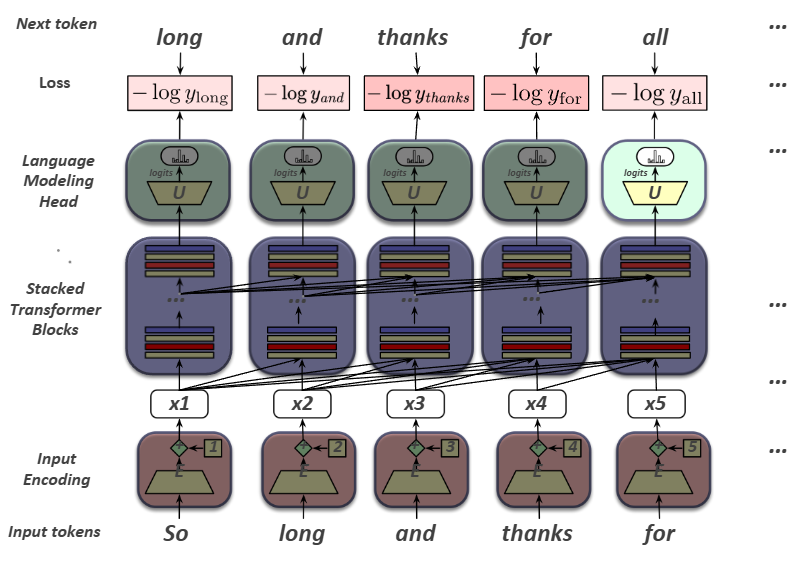
\includegraphics[width=0.9\linewidth]{pic/transformer_language_model_scheme.png}
                \caption{Esquema de treinamento de um modelo de linguagem Transformer.}
                \label{fig:transformer_language_model_scheme}
            \end{figure}
        \end{column}
        \begin{column}{0.4\textwidth}
            \[ \text{Perda Total do Lote} = \frac{1}{T} \sum_{t=1}^{T} L_{CE} \]
        \end{column}
    \end{columns}
\end{frame}

%%%%%%%%%%%%%%%%%%%%%%%%%%%%%%%%%%%%%%%%%%%%%%%%%%
\section{Eng. de Dados e Aj. Fino}

\begin{frame}{Os LLMs são treinados principalmente na web}\justifying
    \begin{itemize}
        \item \textbf{Common Crawl:} Instantâneos massivos de toda a web pública produzidos recursivamente pela organização sem fins lucrativos Common Crawl, contendo bilhões de páginas HTML brutas.
        \item \textbf{Colossal Clean Crawled Corpus (C4):} Criado por Raffel et al. (2020), este conjunto de dados contém 156 bilhões de tokens de texto em inglês que foram rigorosamente filtrados por qualidade.
        \item \textbf{O que constitui esses dados?} A maior parte dos tokens de alta qualidade deriva de documentos de patentes, bancos de dados da Wikipedia e sites de notícias internacionais.
    \end{itemize}
\end{frame}

\begin{frame}{The Pile: um corpus de pré-treinamento projetado}\justifying
    Um conjunto de dados de modelagem de linguagem de código aberto de 825 GiB diversificado e meticulosamente balanceado.
    \vspace{0.5cm}
    \begin{table}
        \centering
        \begin{tabular}{lll}
            \toprule
            \textbf{Acadêmico} & \textbf{Web \& Geral} & \textbf{Livros \& Diálogos} \\
            \midrule
            PubMed Central & Pile-CC & Bibliotik \\
            ArXiv & OpenWebText2 & PG-19 \\
            FreeLaw & StackExchange & BookCorpus2 \\
            PhilPapers & Wikipedia & Ubuntu IRC / GitHub \\
            \bottomrule
        \end{tabular}
    \end{table}
\end{frame}

\begin{frame}{O que um modelo aprende no pré-treinamento?}\justifying
    O texto bruto ingerido contém uma enorme quantidade de conhecimento humano. O pré-treinamento com bilhões de textos contendo todo esse conhecimento é o que fundamentalmente dá aos modelos de linguagem sua capacidade de executar tanta lógica.
    \begin{itemize}
        \item Lógica Contextual: "Há caninos por toda parte! Um cachorro na sala da frente e dois cachorros."
        \item Escalonamento Semântico: "Não era apenas grande, era enorme."
        \item Recuperação Factual: "A autora de 'Um Teto Todo Seu' é Virginia Woolf."
        \item Verdades Matemáticas: "A raiz quadrada de 4 é 2."
    \end{itemize}
\end{frame}

\begin{frame}{Ajuste fino como "pré-treinamento contínuo"}\justifying
    \begin{itemize}
        \item A abordagem mais direta é treinar ainda mais todos os bilhões de parâmetros do modelo nos novos dados específicos.
        \item Empregamos exatamente o mesmo método (previsão da próxima palavra) e função de perda matemática (perda de entropia cruzada) utilizados para o pré-treinamento original.
        \item Tratamos a operação como se os novos dados especializados fossem simplesmente anexados no final da sequência massiva de dados de pré-treinamento.
        \item Portanto, esse processo é frequentemente classificado na literatura como \textbf{pré-treinamento contínuo}.
    \end{itemize}
\end{frame}

\begin{frame}{Ajuste fino}\justifying
    \begin{figure}
        \centering
        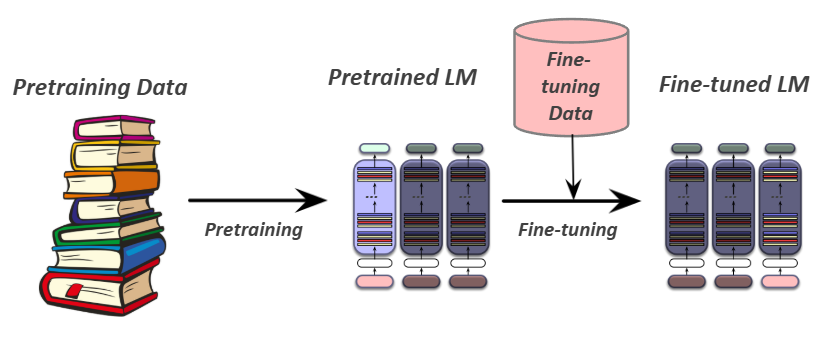
\includegraphics[width=\linewidth]{pic/finetuning.png}
        \caption{Finetuning flow}
        \label{fig:finetuning_flow}
    \end{figure}
\end{frame}

%%%%%%%%%%%%%%%%%%%%%%%%%%%%%%%%%%%%%%%%%%%%%%%%%%
\section{Ava., Leis de Escala e Otimização}

\begin{frame}{Avaliando Grandes Modelos de Linguagem}
    \begin{center}
        \huge \textbf{Avaliando Grandes Modelos de Linguagem}\\
        \vspace{0.5cm}
        \Large Métricas e Infraestrutura de Escala.
    \end{center}
\end{frame}

\begin{frame}{Métrica de Perplexidade}\justifying
    A indústria usa a Perplexidade para medir matematicamente quão bem o LM prevê distribuições de texto não vistas. \\
    \vspace{0.3cm}
    A perplexidade de um modelo em um conjunto de teste não visto é definida como o inverso da probabilidade que o modelo atribui ao conjunto de teste, normalizada geometricamente pelo comprimento do conjunto de teste. \\
    \vspace{0.3cm}
    Para uma sequência de teste de $n$ tokens $w_{1:n}$, a perplexidade é calculada como:
    \[ \text{Perplexidade}(w_{1:n}) = P(w_{1:n})^{-\frac{1}{n}} \]
\end{frame}

\begin{frame}{Por que perplexidade em vez de probabilidade bruta?}\justifying
    \begin{itemize}
        \item A probabilidade bruta depende inteiramente do tamanho do conjunto de teste; a probabilidade se torna assintoticamente menor quanto mais longa for a sequência de texto.
        \item A perplexidade calcula a probabilidade inversa normalizada pelo número total de palavras (derivada da taxa de entropia cruzada).
        \item Enquanto a probabilidade opera em uma faixa estreita de $[0, 1]$, a faixa de perplexidade abrange $[1, \infty]$.
        \item Quanto maior a probabilidade atribuída à sequência de palavras, menor a perplexidade.
    \end{itemize}
\end{frame}

\begin{frame}{Leis de Escala}\justifying
    O desempenho empírico do LLM é estritamente dependente de:
    \begin{itemize}
        \item \textbf{Tamanho do modelo:} Número absoluto de parâmetros treináveis.
        \item \textbf{Tamanho do conjunto de dados:} A quantidade volumétrica bruta de dados.
        \item \textbf{Computação:} Quantidade absoluta de computação utilizada.
    \end{itemize}
    O desempenho de um grande modelo de linguagem (medido pela perda) escala matematicamente como uma lei de potência:
    \[ L(N) = (N_c/N)^{\alpha_N} \quad L(D) = (D_c/D)^{\alpha_D} \quad L(C) = (C_c/C)^{\alpha_C} \]
\end{frame}

\begin{frame}{Número de parâmetros não-embedding N}\justifying
    Podemos estimar matematicamente o total de parâmetros via:
    \[ N \approx 2 d_{model} n_{layers} (2d_{attn} + d_{ff}) \]   
    \[ \approx 12 n_{layers} d_{model}^2 \]
    Assumindo proporções dimensionais padrão de $d_{attn} = d_{ff}/4 = d_{model}$. \\
    \vspace{0.5cm}
    Assim, calculando para a arquitetura do GPT-3, possuindo $n=96$ camadas e uma dimensionalidade massiva de $d=12288$, determinamos:
    \[ 12 \times 96 \times 12288^2 \approx 175 \text{ bilhões de parâmetros.} \]
\end{frame}

\begin{frame}{O Gargalo do Cache KV}\justifying
    Durante a fase de pré-treinamento, calculamos a atenção matemática com eficiência em lotes paralelos massivos. Porém, isso falha na inferência, pois geramos tokens sequencialmente.
    \begin{itemize}
        \item Para cada novo token $x$, multiplicamos pelas matrizes de peso $W_Q, W_K, W_V$.
        \item O cálculo exige vetores chave e valor para todos os tokens anteriores $x_{<i}$, gerando um custo computacional $O(N^2)$.
        \item \textbf{A Solução de Engenharia:} Armazene os vetores na memória VRAM da GPU no cache KV, para uso com velocidade de inferência $O(N)$.
    \end{itemize}
\end{frame}

\begin{frame}{Arquitetura do Cache KV}\justifying
    \begin{figure}
        \centering
        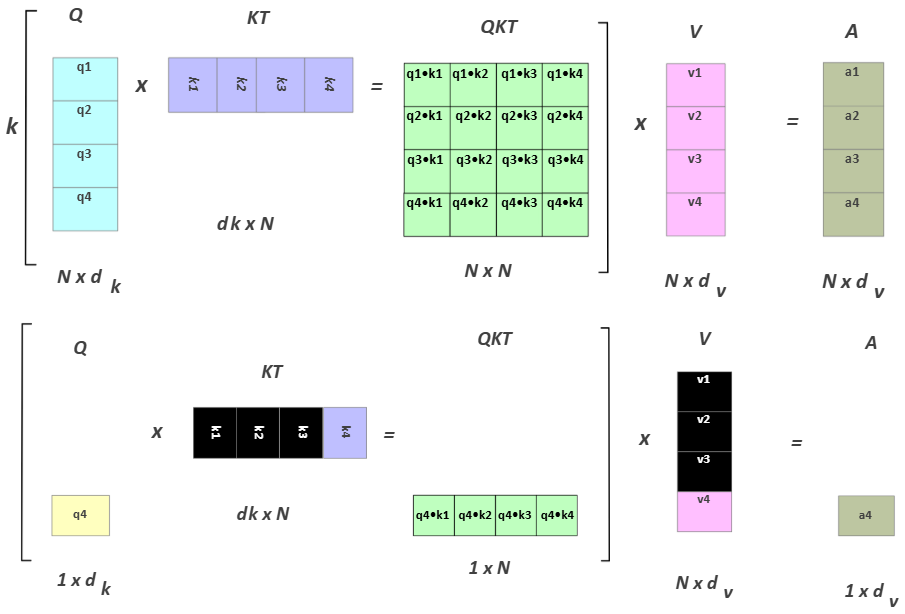
\includegraphics[width=0.6\linewidth]{pic/kv_cache.png}
        \caption{Representação do cache KV.}
        \label{fig:kv_cache_representation}
    \end{figure}
\end{frame}

\begin{frame}{Teoria LORA (Adaptação de Baixo Posto)}\justifying
    Considere uma matriz de pesos base $W$ ($N \times d$) que teoricamente precisa ser atualizada durante o ajuste fino. No algoritmo LORA, congelamos $W$ e atualizamos uma decomposição de baixo posto de $W$:
    \begin{itemize}
        \item Matriz $A$ com formato $N \times r$
        \item Matriz $B$ com formato $r \times d$
        \item Onde $r$ (posto) é muito pequeno (ex: 1, 2 ou 8)
    \end{itemize}
    Substituímos computacionalmente $W + \Delta W$ por $W + BA$. \\
    Passagem direta (Forward pass):
    \[ h = xW + xAB \]
\end{frame}

%%%%%%%%%%%%%%%%%%%%%%%%%%%%%%%%%%%%%%%%%%%%%%%%%%
\section{Danos e Referências}

\begin{frame}{Danos Sociais dos Grandes Modelos de Linguagem}\justifying
    \begin{itemize}
        \item \textbf{Alucinação}
        \item \textbf{Litígio de Direitos Autorais}
        \item \textbf{Violações de Privacidade}
        \item \textbf{Toxicidade e Exploração}
        \item \textbf{Desinformação Política}
    \end{itemize}
\end{frame}

\begin{frame}{Alucinação}
    Chatbots rotineiramente 'alucinam' políticas corporativas falsas ou fatos inexistentes.
    \vspace{0.5cm}
    
    \begin{figure}
      \centering
      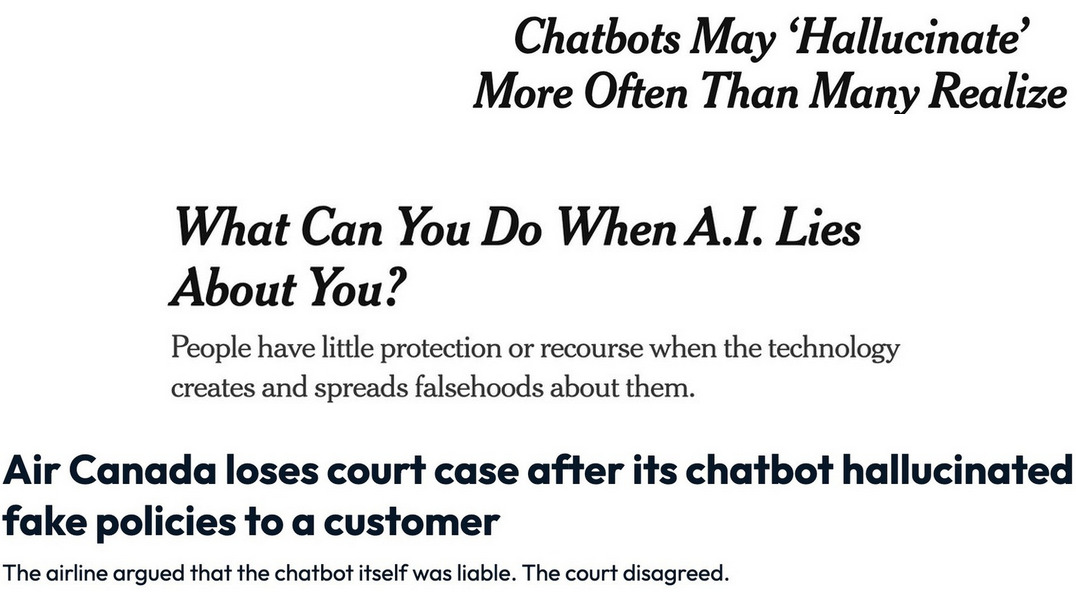
\includegraphics[width=0.5\linewidth]{pic/hallucination.jpeg}
    \end{figure}
\end{frame}

\begin{frame}{Litígio de Direitos Autorais}
    Ações judiciais por infração massiva no uso de obras protegidas durante o treinamento sem permissão.
    \vspace{0.5cm}
    
    \begin{figure}
      \centering
      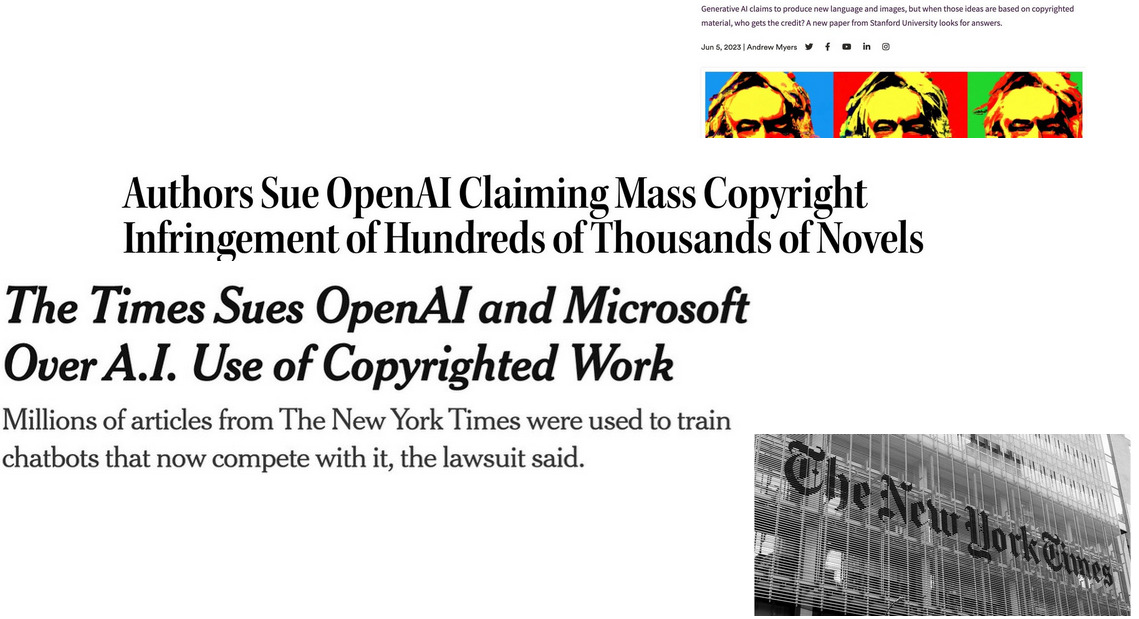
\includegraphics[width=0.5\linewidth]{pic/copyright-litigation.jpeg}
    \end{figure}
\end{frame}

\begin{frame}{Violações de Privacidade}
    Vazamento acidental de e-mails e números de telefone privados extraídos dos dados de treinamento.
    \vspace{0.5cm}
    
    \begin{figure}
      \centering
      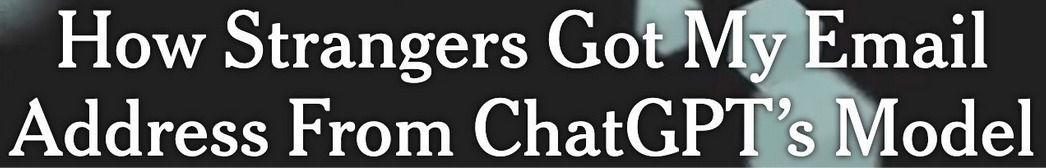
\includegraphics[width=0.6\linewidth]{pic/privacy-breaches.jpeg}
    \end{figure}
\end{frame}

\begin{frame}{Toxicidade e Exploração}
    O processo de limpeza dos dados muitas vezes exige que humanos avaliem conteúdos tóxicos.
    \vspace{0.5cm}
    
    \begin{figure}
      \centering
      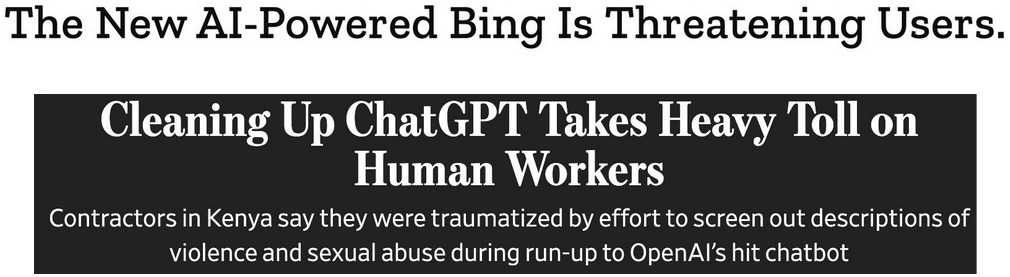
\includegraphics[width=0.6\linewidth]{pic/toxicity-and-exploitation.jpeg}
    \end{figure}
\end{frame}

\begin{frame}{Desinformação Política}
    Geração de falsidades altamente persuasivas que podem afetar cenários globais e eleições.
    \vspace{0.5cm}
    
    \begin{figure}
        \centering
        
\includegraphics[width=0.6\linewidth]{pic/political-misinformation.jpeg}
    \end{figure}
\end{frame}

\begin{frame}[allowframebreaks]{Referências Bibliográficas}\justifying
    \begin{thebibliography}{99}
    {\scriptsize
    
    \bibitem{anthropic2025} Anthropic. 2025. Release notes: System prompts. \url{https://docs.anthropic.com/en/release-notes/system-prompts}.
    
    \bibitem{bellegarda1997} Bellegarda, J. R. 1997. A latent semantic analysis framework for large-span language modeling. EUROSPEECH.
    
    \bibitem{bengio2000} Bengio, Y., R. Ducharme, and P. Vincent. 2000. A neural probabilistic language model. NeurIPS.
    
    \bibitem{bengio2003} Bengio, Y., R. Ducharme, P. Vincent, and C. Jauvin. 2003. A neural probabilistic language model. JMLR, 3:1137–1155.
    
    \bibitem{bengio2006} Bengio, Y., H. Schwenk, J.-S. Sen\'ecal, F. Morin, and J.-L. Gauvain. 2006. Neural probabilistic language models. In Innovations in Machine Learning, 137–186. Springer.
    
    \bibitem{bickmore2018} Bickmore, T. W., et al. 2018. Patient and consumer safety risks when using conversational assistants for medical information. Journal of Medical Internet Research, 20(9):e11510.
    
    \bibitem{blodgett2020} Blodgett, S. L., S. Barocas, H. Daum\'e III, and H. Wallach. 2020. Language (technology) is power: A critical survey of “bias” in NLP. ACL.
    
    \bibitem{bommasani2021} Bommasani, R., et al. 2021. On the opportunities and risks of foundation models. ArXiv.
    
    \bibitem{brown2020} Brown, T., et al. 2020. Language models are few-shot learners. NeurIPS, 33.
    
    \bibitem{carlini2021} Carlini, N., et al. 2021. Extracting training data from large language models. USENIX Security 21.
    
    \bibitem{cheng2023} Cheng, M., E. Durmus, and D. Jurafsky. 2023. Marked personas: Using natural language prompts to measure stereotypes in language models. ACL.
    
    \bibitem{cheng2025} Cheng, M., et al. 2025. Sycophantic ai decreases prosocial intentions and promotes dependence. ArXiv preprint.
    
    \bibitem{coccaro1998} Coccaro, N. and D. Jurafsky. 1998. Towards better integration of semantic predictors in statistical language modeling. ICSLP.
    
    \bibitem{dai2015} Dai, A. M. and Q. V. Le. 2015. Semi-supervised sequence learning. NeurIPS.
    
    \bibitem{deerwester1988} Deerwester, S. C., et al. 1988. Computer information retrieval using latent semantic structure: US Patent 4,839,853.
    
    \bibitem{devlin2019} Devlin, J., M.-W. Chang, K. Lee, and K. Toutanova. 2019. BERT: Pre-training of deep bidirectional transformers for language understanding. NAACL HLT.
    
    \bibitem{dinan2020} Dinan, E., et al. 2020. Queens are powerful too: Mitigating gender bias in dialogue generation. EMNLP.
    
    \bibitem{dinan2021} Dinan, E., et al. 2021. Anticipating safety issues in e2e conversational ai: Framework and tooling. ArXiv.
    
    \bibitem{dodge2019} Dodge, J., et al. 2019. Show your work: Improved reporting of experimental results. EMNLP.
    
    \bibitem{dodge2021} Dodge, J., et al. 2021. Documenting large webtext corpora: A case study on the colossal clean crawled corpus. EMNLP.
    
    \bibitem{ethayarajh2020} Ethayarajh, K. and D. Jurafsky. 2020. Utility is in the eye of the user: A critique of NLP leaderboards. EMNLP.
    
    \bibitem{friedman2017} Friedman, B., D. G. Hendry, and A. Borning. 2017. A survey of value sensitive design methods. Foundations and Trends in Human-Computer Interaction.
    
    \bibitem{friedman2019} Friedman, B. and D. G. Hendry. 2019. Value Sensitive Design: Shaping Technology with Moral Imagination. MIT Press.
    
    \bibitem{gao2020} Gao, L., et al. 2020. The Pile: An 800GB dataset of diverse text for language modeling. ArXiv.
    
    \bibitem{gehman2020} Gehman, S., S. Gururangan, M. Sap, Y. Choi, and N. A. Smith. 2020. RealToxicityPrompts: Evaluating neural toxic degeneration in language models. Findings of EMNLP.
    
    \bibitem{gururangan2020} Gururangan, S., et al. 2020. Don’t stop pretraining: Adapt language models to domains and tasks. ACL.
    
    \bibitem{hashimoto2018} Hashimoto, T., M. Srivastava, H. Namkoong, and P. Liang. 2018. Fairness without demographics in repeated loss minimization. ICML.
    
    \bibitem{heafield2011} Heafield, K. 2011. KenLM: Faster and smaller language model queries. Workshop on Statistical Machine Translation.
    
    \bibitem{henderson2017} Henderson, P., et al. 2017. Ethical challenges in data-driven dialogue systems. AAAI/ACM AI Ethics and Society Conference.
    
    \bibitem{henderson2020} Henderson, P., et al. 2020. Towards the systematic reporting of the energy and carbon footprints of machine learning. JMLR.
    
    \bibitem{henderson2023} Henderson, P., et al. 2023. Foundation models and fair use. JMLR, 24(400):1–79.
    
    \bibitem{hofmann2024} Hofmann, V., P. R. Kalluri, D. Jurafsky, and S. King. 2024. Ai generates covertly racist decisions about people based on their dialect. Nature, 633(8028):147–154.
    
    \bibitem{ischen2019} Ischen, C., et al. 2019. Privacy concerns in chatbot interactions. International Workshop on Chatbot Research and Design.
    
    \bibitem{jelinek1975} Jelinek, F., R. L. Mercer, and L. R. Bahl. 1975. Design of a linguistic statistical decoder for the recognition of continuous speech. IEEE Transactions on Information Theory.
    
    \bibitem{khattab2024} Khattab, O., et al. 2024. DSPy: Compiling declarative language model calls into self-improving pipelines. ICLR.
    
    \bibitem{kiela2021} Kiela, D., et al. 2021. Dynabench: Rethinking benchmarking in NLP. NAACL HLT.
    
    \bibitem{landauer1997} Landauer, T. K., D. Laham, B. Rehder, and M. E. Schreiner. 1997. How well can passage meaning be derived without using word order? COGSCI.
    
    \bibitem{liang2023} Liang, P., et al. 2023. Holistic evaluation of language models. Transactions on Machine Learning Research.
    
    \bibitem{liu2020} Liu, H., et al. 2020. Does gender matter? Towards fairness in dialogue systems. COLING.
    
    \bibitem{llama2024} Llama Team. 2024. The llama 3 herd of models.
    
    \bibitem{longpre2024a} Longpre, S., et al. 2024a. Consent in crisis: The rapid decline of the ai data commons. ArXiv preprint.
    
    \bibitem{longpre2024b} Longpre, S., et al. 2024b. A pretrainer’s guide to training data: Measuring the effects of data age, domain coverage, quality, \& toxicity. NAACL HLT.
    
    \bibitem{mcguffie2020} McGuffie, K. and A. Newhouse. 2020. The radicalization risks of GPT-3 and advanced neural language models. ArXiv.
    
    \bibitem{mikolov2010} Mikolov, T., et al. 2010. Recurrent neural network based language model. INTERSPEECH.
    
    \bibitem{mikolov2011} Mikolov, T., et al. 2011. Extensions of recurrent neural network language model. ICASSP.
    
    \bibitem{mikolov2013a} Mikolov, T., K. Chen, G. S. Corrado, and J. Dean. 2013a. Efficient estimation of word representations in vector space. ICLR.
    
    \bibitem{mikolov2013b} Mikolov, T., I. Sutskever, K. Chen, G. S. Corrado, and J. Dean. 2013b. Distributed representations of words and phrases and their compositionality. NeurIPS.
    
    \bibitem{miller1950} Miller, G. A. and J. A. Selfridge. 1950. Verbal context and the recall of meaningful material. American Journal of Psychology, 63:176–185.
    
    \bibitem{min2022} Min, S., et al. 2022. Rethinking the role of demonstrations: What makes in-context learning work? EMNLP.
    
    \bibitem{nadeem2021} Nadeem, M., A. Bethke, and S. Reddy. 2021. StereoSet: Measuring stereotypical bias in pretrained language models. ACL.
    
    \bibitem{neff2016} Neff, G. and P. Nagy. 2016. Talking to bots: Symbiotic agency and the case of Tay. International Journal of Communication.
    
    \bibitem{parrish2022} Parrish, A., et al. 2022. BBQ: A hand-built bias benchmark for question answering. Findings of ACL 2022.
    
    \bibitem{peters2018} Peters, M., et al. 2018. Deep contextualized word representations. NAACL HLT.
    
    \bibitem{radford2019} Radford, A., et al. 2019. Language models are unsupervised multitask learners. OpenAI tech report.
    
    \bibitem{raffel2020} Raffel, C., et al. 2020. Exploring the limits of transfer learning with a unified text-to-text transformer. JMLR, 21(140):1–67.
    
    \bibitem{rawls2001} Rawls, J. 2001. Justice as fairness: A restatement. Harvard University Press.
    
    \bibitem{reeves1996} Reeves, B. and C. Nass. 1996. The Media Equation: How People Treat Computers, Television, and New Media Like Real People and Places. Cambridge University Press.
    
    \bibitem{rosenfeld1992} Rosenfeld, R. 1992. Adaptive Statistical Language Modeling: A Maximum Entropy Approach. Ph.D. thesis, Carnegie Mellon University.
    
    \bibitem{rosenfeld1996} Rosenfeld, R. 1996. A maximum entropy approach to adaptive statistical language modeling. Computer Speech and Language, 10:187–228.
    
    \bibitem{sagawa2020} Sagawa, S., P. W. Koh, T. B. Hashimoto, and P. Liang. 2020. Distributionally robust neural networks for group shifts: On the importance of regularization for worst-case generalization. ICLR.
    
    \bibitem{shannon1948} Shannon, C. E. 1948. A mathematical theory of communication. Bell System Technical Journal, 27(3):379–423.
    
    \bibitem{sheng2019} Sheng, E., K.-W. Chang, P. Natarajan, and N. Peng. 2019. The woman worked as a babysitter: On biases in language generation. EMNLP.
    
    \bibitem{soldaini2024} Soldaini, L., et al. 2024. Dolma: An open corpus of three trillion tokens for language model pretraining research. ArXiv.
    
    \bibitem{stolcke2002} Stolcke, A. 2002. SRILM – an extensible language modeling toolkit. ICSLP.
    
    \bibitem{strubell2019} Strubell, E., A. Ganesh, and A. McCallum. 2019. Energy and policy considerations for deep learning in NLP. ACL.
    
    \bibitem{vaswani2017} Vaswani, A., et al. 2017. Attention is all you need. NeurIPS.
    
    \bibitem{webson2022} Webson, A. and E. Pavlick. 2022. Do prompt-based models really understand the meaning of their prompts? NAACL HLT.
    
    \bibitem{weizenbaum1966} Weizenbaum, J. 1966. ELIZA – A computer program for the study of natural language communication between man and machine. CACM.
    
    \bibitem{wolf2017} Wolf, M. J., K. W. Miller, and F. S. Grodzinsky. 2017. Why we should have seen that coming: Comments on Microsoft’s Tay “experiment,” and wider implications. The ORBIT Journal.
    
    \bibitem{xu2020} Xu, J., et al. 2020. Recipes for safety in open-domain chatbots. ArXiv.
    
    \bibitem{xu2021} Xu, A., et al. 2021. Detoxifying language models risks marginalizing minority voices. NAACL HLT.
    
    \bibitem{zaosanders2025} Zao-Sanders, M. 2025. How People Are Really Using Gen AI in 2025 — hbr.org. \url{https://hbr.org/2025/04/how-people-are-really-using-gen-ai-in-2025}.
    
    \bibitem{zhang2025} Zhang, A. K., et al. 2025. Language model developers should report train-test overlap. ICML.
    
    }
    \end{thebibliography}
\end{frame}

%%%%%%%%%%%%%%%%%%%%%%%%%%%%%%%%%%%%%%%%%%%%%%%%%%
\begin{frame}
    \begin{center}
        \Large \textbf{OBRIGADO}
    \end{center}
\end{frame}
%%%%%%%%%%%%%%%%%%%%%%%%%%%%%%%%%%%%%%%%%%%%%%%%%%
\end{document}